\chapter{Regressão Linear}
\label{cap:regressao}

A regressão linear estuda a relação entre uma resposta contínua e uma ou mais variáveis explicativas. Na regressão simples, usamos um preditor; na múltipla, usamos vários. Vamos começar pela relação entre horas de estudo e nota posterior no arquivo fictício \texttt{exemplo\_notas.csv}.

A pergunta desta seção é: como a nota média se relaciona com as horas de estudo \textbf{no modelo ajustado}? Ela não é equivalente a perguntar quanto a nota de uma pessoa aumentaria se ela fosse obrigada a estudar uma hora a mais. A segunda pergunta envolve uma interpretação causal que a reta, isoladamente, não fornece.

\section{Correlação e regressão}

A correlação de Pearson resume a direção e a intensidade da associação linear entre duas variáveis. Ela é simétrica: trocar a ordem das variáveis não muda o coeficiente. Já a regressão distingue uma resposta de seus preditores e expressa uma relação nas unidades dessas variáveis.

O jamovi oferece Pearson, Spearman e Kendall na \textbf{Matriz de correlação (Correlation Matrix)}, no grupo de análises de \textbf{Regressão}. Solicite o número de casos e intervalos quando forem pertinentes \parencite{JamoviCorrelacao}. Spearman trabalha com postos e pode descrever associações monotônicas; não é simplesmente um botão que resolve qualquer dificuldade de distribuição ou de desenho.

Uma correlação de Pearson próxima de zero não exclui toda relação possível: duas variáveis podem ter uma associação curva e correlação linear pequena. Por isso, examine um gráfico de dispersão antes de resumir a relação em um único coeficiente.

\subsection{Calculando e interpretando uma correlação}

Para pares completos $(x_i,y_i)$, o coeficiente de Pearson é:
\[
r=\frac{\sum_i(x_i-\bar x)(y_i-\bar y)}
{\sqrt{\sum_i(x_i-\bar x)^2\sum_i(y_i-\bar y)^2}}.
\]
O numerador acompanha a covariação: pessoas acima da média em horas e acima da média em nota contribuem com um produto positivo. O denominador padroniza a escala. Assim, $r$ não tem unidade e permanece igual se trocarmos horas por minutos mediante uma transformação linear positiva. Trocar a unidade muda a inclinação da regressão, como veremos adiante.

Para \texttt{horas} e \texttt{depois}, obtemos $r\approx0{,}840$, em 18 pares. Na inferência usual de Pearson para pares independentes sob um modelo normal bivariado, o teste de $H_0:\rho=0$ usa:
\[
t=r\sqrt{\frac{n-2}{1-r^2}},\qquad gl=n-2.
\]
Neste caso, $t\approx6{,}183$, com 16 graus de liberdade. O parâmetro $\rho$ é a correlação populacional; $r$ é sua estimativa. A documentação de \texttt{cor.test} apresenta esse teste e o intervalo aproximado por transformação de Fisher \parencite{RCorrelacao}. Para o exemplo, o IC95\% por esse método é aproximadamente $[0{,}613;0{,}939]$.

A relação positiva é clara nos dados construídos, mas o intervalo não autoriza tratá-la como uma constante exata da população. Também não significa que uma pessoa estude mais \textit{porque} sua nota é alta ou que uma mudança nas horas produza necessariamente a mudança prevista na nota. Amostragem, desenho e variáveis omitidas continuam relevantes.

\subsection{Uma relação forte pode ter correlação zero}

Considere os cinco pares $(-2,4)$, $(-1,1)$, $(0,0)$, $(1,1)$ e $(2,4)$. Eles seguem exatamente $y=x^2$. Os produtos centrados se compensam, e a correlação de Pearson é zero. A figura~\ref{fig:correlacao-curva} mostra por que a expressão ``sem relação'' seria inadequada para descrever esse conjunto.

\begin{figure}[H]
\centering
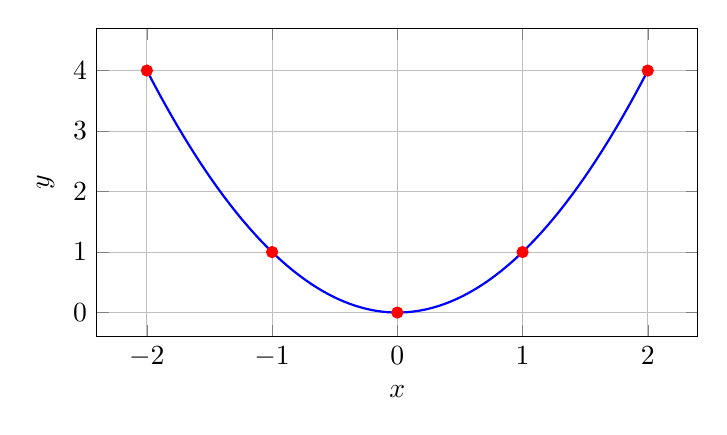
\begin{tikzpicture}
\begin{axis}[
  width=0.76\textwidth,height=5.5cm,
  xlabel={$x$},ylabel={$y$},xmin=-2.4,xmax=2.4,ymin=-0.4,ymax=4.7,
  xtick={-2,-1,0,1,2},ytick={0,1,2,3,4},grid=major
]
  \addplot[blue,thick,domain=-2:2,samples=80] {x*x};
  \addplot[only marks,mark=*,red] coordinates {(-2,4) (-1,1) (0,0) (1,1) (2,4)};
\end{axis}
\end{tikzpicture}
\caption{Cinco pares construídos com relação quadrática perfeita e correlação de Pearson zero. A curva descreve uma relação que não é linear nem monotônica em todo o intervalo. Elaboração própria.}
\label{fig:correlacao-curva}
\end{figure}

Spearman também não transforma toda relação curva em uma associação monotônica: neste exemplo simétrico, os postos não crescem continuamente de um extremo ao outro. Escolher Pearson ou Spearman começa pela relação que queremos descrever. Confira a dispersão, os empates, os limites da escala e observações influentes antes de interpretar o coeficiente.

\subsection{Quantas pessoas há em cada correlação?}

Em uma matriz com $k$ variáveis, existem $k(k-1)/2$ pares distintos: seis variáveis produzem 15 correlações. Esse número ajuda a reconhecer a multiplicidade quando todos os testes são examinados. Se as perguntas forem exploratórias, apresente a matriz completa e sua finalidade; se forem confirmatórias, defina as comparações principais e o ajuste pertinente, retomando o capítulo~\ref{cap:hipoteses}.

Solicite o número de casos no painel de correlação \parencite{JamoviCorrelacao}. Com ausentes, diferentes pares podem utilizar pessoas diferentes. O coeficiente de horas com nota anterior e o de horas com nota posterior podem então refletir, além de associações distintas, alterações na composição da amostra. Registre a regra efetivamente usada e confira a amostra antes de comparar coeficientes ou combiná-los em outros modelos.

\section{O modelo de uma reta}

Escrevemos o modelo simples como:
\[
Y_i=\beta_0+\beta_1X_i+\varepsilon_i.
\]
Aqui, $Y_i$ é a nota da pessoa $i$, $X_i$ é o número de horas de estudo, $\beta_0$ é o intercepto e $\beta_1$ é a inclinação. O termo $\varepsilon_i$ representa a parte da resposta não descrita pela média condicional modelada.

Depois do ajuste, usamos coeficientes estimados e obtemos uma previsão da média, $\widehat{Y}_i=\widehat{\beta}_0+\widehat{\beta}_1X_i$. O resíduo é a diferença entre o observado e o ajustado: $e_i=Y_i-\widehat{Y}_i$. O método dos mínimos quadrados escolhe os coeficientes que minimizam a soma dos quadrados desses resíduos \parencite{NISTRegressao}.

\section{Ajustando a regressão no jamovi}

\begin{enumerate}
  \item Abra \texttt{exemplo\_notas.csv} e desative os filtros. Confira que as colunas \texttt{horas} e \texttt{depois} estão como contínuas.
  \item Acesse \textbf{Análises $\rightarrow$ Regressão $\rightarrow$ Regressão linear (Linear Regression)}.
  \item Atribua \texttt{depois} à \textbf{Variável dependente (Dependent Variable)} e \texttt{horas} às \textbf{Covariáveis (Covariates)}. Mantenha o intercepto no modelo.
  \item Solicite o intervalo de confiança dos coeficientes e examine as medidas de ajuste. Nos diagnósticos, peça o gráfico Q-Q dos resíduos e os gráficos de resíduos.
\end{enumerate}

As opções de coeficientes, ajuste, resíduos e medidas de influência são documentadas pelo projeto jamovi \parencite{JamoviRegressao}. Os nomes de algumas opções podem aparecer em inglês mesmo quando outros menus estão traduzidos.

\subsection{Conferindo a equação e as unidades}

O ajuste aos 18 casos fictícios resulta aproximadamente em:
\[
\widehat{\text{nota posterior}}=49{,}764+5{,}221\times\text{horas}.
\]
No modelo simples, uma hora adicional está associada a um aumento de aproximadamente $5{,}22$ pontos na nota média ajustada. O coeficiente tem unidade de pontos por hora. Para três horas, a previsão da média é aproximadamente $65{,}43$ pontos.

O intercepto é a previsão quando \texttt{horas} vale zero. Como o banco contém apenas valores de uma a cinco horas, sua interpretação prática em zero exige extrapolação. Não confunda a existência de um intercepto na equação com evidência observada sobre pessoas que estudaram zero horas.

\begin{figure}[H]
\centering
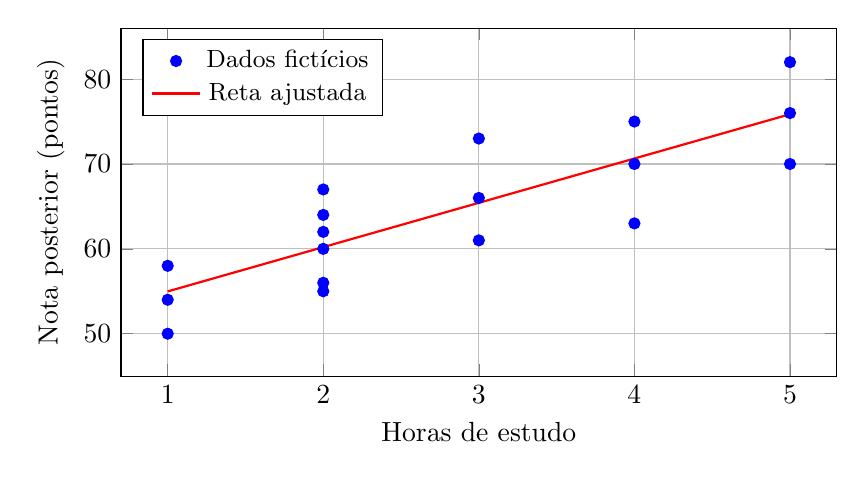
\begin{tikzpicture}
\begin{axis}[
  width=0.88\textwidth,height=6cm,
  xlabel={Horas de estudo},ylabel={Nota posterior (pontos)},
  xmin=0.7,xmax=5.3,ymin=45,ymax=86,
  xtick={1,2,3,4,5},grid=major,
  legend style={at={(0.03,0.97)},anchor=north west,font=\small}
]
  \addplot[only marks,mark=*,blue] coordinates {
    (1,50) (2,56) (2,55) (3,61) (4,63) (5,70)
    (1,54) (2,60) (2,62) (3,66) (4,70) (5,76)
    (1,58) (2,64) (2,67) (3,73) (4,75) (5,82)
  };
  \addlegendentry{Dados fictícios}
  \addplot[red,thick,domain=1:5,samples=2] {49.76410256+5.22051282*x};
  \addlegendentry{Reta ajustada}
\end{axis}
\end{tikzpicture}
\caption{Regressão simples de nota posterior em horas de estudo. Pontos e reta calculados a partir do CSV da apostila; elaboração própria.}
\label{fig:regressao-notas}
\end{figure}

\subsection{O que o R quadrado informa}

Para esse ajuste com intercepto, $R^2\approx0{,}705$. Isso significa que a reta descreve cerca de 70,5\% da soma de quadrados da variação observada das notas em torno da média amostral. Não significa que ela acerte 70,5\% das pessoas nem que as horas tenham causado essa fração das notas.

Ao acrescentar preditores, o $R^2$ do ajuste por mínimos quadrados não diminui, mesmo quando a nova variável acrescenta pouco conhecimento. Por isso, examine também a pergunta, a incerteza dos coeficientes, o número de parâmetros, o $R^2$ ajustado e os diagnósticos. Um modelo mais complexo não é automaticamente mais útil.

\section{Resíduos, pressupostos e limites}

Nos gráficos de resíduos, procure padrões que contrariem o modelo: uma curva pode sugerir forma funcional inadequada; um formato de funil pode indicar variância que muda ao longo dos valores ajustados. O gráfico Q-Q ajuda a examinar a aproximação normal dos erros usada na inferência usual. Essa suposição não exige que o próprio preditor \texttt{horas} tenha distribuição normal.

A independência dos erros também precisa ser justificada pelo desenho. Notas repetidas da mesma pessoa, pessoas da mesma turma ou medições ao longo do tempo podem exigir uma estrutura que a regressão simples não contempla. As ferramentas de diagnóstico não substituem esse conhecimento sobre a coleta.

Observe possíveis casos influentes e confira os registros originais. Um ponto pode ser extremo em uma variável e não ter grande influência sobre a reta, ou pode mudar bastante o ajuste. Não exclua casos apenas para aumentar $R^2$ ou diminuir o valor de $p$.


\subsection{Lendo os resíduos do nosso exemplo}

Um resíduo positivo informa que a nota observada ficou acima da média ajustada; um negativo, abaixo. Para a primeira pessoa, a nota foi 50 e a previsão com uma hora foi $49{,}764+5{,}221\approx54{,}985$. Portanto, $e_1\approx-4{,}985$ pontos. Ele tem a mesma unidade da resposta.

\begin{figure}[H]
\centering
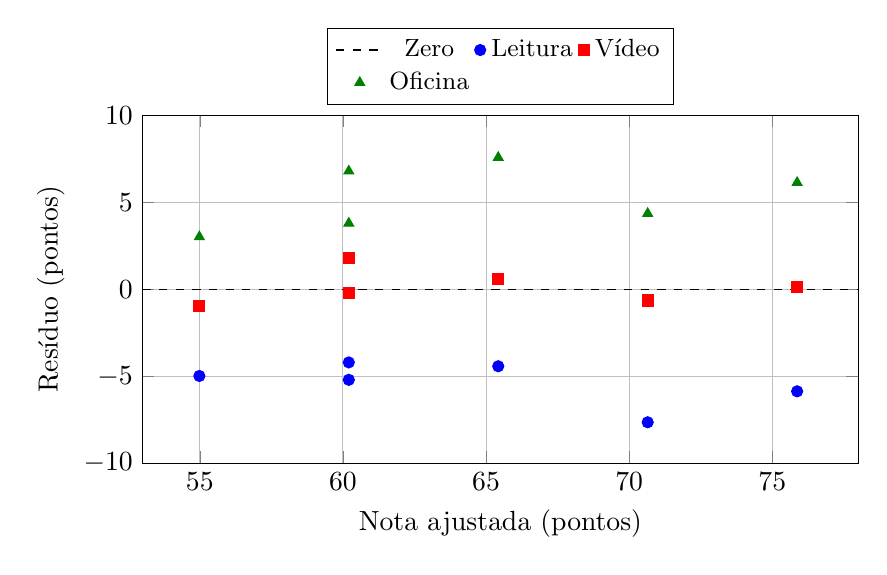
\begin{tikzpicture}
\begin{axis}[
  width=0.88\textwidth,height=6cm,
  xlabel={Nota ajustada (pontos)},ylabel={Resíduo (pontos)},
  xmin=53,xmax=78,ymin=-10,ymax=10,grid=major,
  legend style={at={(0.5,1.03)},anchor=south,legend columns=3,font=\small}
]
  \addplot[black,dashed,domain=53:78,samples=2] {0};
  \addlegendentry{Zero}
  \addplot[only marks,blue,mark=*] coordinates {
    (54.984615,-4.984615) (60.205128,-4.205128) (60.205128,-5.205128)
    (65.425641,-4.425641) (70.646154,-7.646154) (75.866667,-5.866667)};
  \addlegendentry{Leitura}
  \addplot[only marks,red,mark=square*] coordinates {
    (54.984615,-0.984615) (60.205128,-0.205128) (60.205128,1.794872)
    (65.425641,0.574359) (70.646154,-0.646154) (75.866667,0.133333)};
  \addlegendentry{Vídeo}
  \addplot[only marks,green!50!black,mark=triangle*] coordinates {
    (54.984615,3.015385) (60.205128,3.794872) (60.205128,6.794872)
    (65.425641,7.574359) (70.646154,4.353846) (75.866667,6.133333)};
  \addlegendentry{Oficina}
\end{axis}
\end{tikzpicture}
\caption{Resíduos do modelo simples nota posterior em horas, identificados por grupo. O modelo não incluiu o grupo: a figura ajuda a perceber uma estrutura que a reta única deixa nos resíduos. Elaboração própria a partir do CSV.}
\label{fig:residuos-notas}
\end{figure}

Todos os resíduos de Leitura são negativos, enquanto os de Oficina são positivos. Isso sugere examinar como o grupo participa da pergunta e do modelo, em vez de considerar somente o $R^2=0{,}705$. Um diagnóstico indica algo a investigar; não decide sozinho qual interpretação causal atribuir ao grupo. O NIST destaca o papel dos gráficos de resíduos na avaliação de modelos \parencite{NISTDiagnostico}.

No ajuste por mínimos quadrados com intercepto, os resíduos somam zero, salvo arredondamento. Isso acontece pela própria estimação e \textbf{não comprova} normalidade, independência ou ausência de viés de seleção. Os erros $\varepsilon_i$ do modelo não são observados diretamente; os resíduos são calculados após estimar os parâmetros.

Para interpretar a reta como média condicional, especificamos $E(\varepsilon_i\mid X_i)=0$ no modelo simples; na múltipla, a condição envolve o conjunto de preditores. Homogeneidade da variância e normalidade dos erros entram na inferência clássica correspondente. Uma reta pode ser calculada mesmo quando essas condições não são adequadas; conseguir um resultado numérico não encerra sua avaliação.

\section{Regressão múltipla: incluindo a nota anterior}
\label{sec:regressao-multipla}

Vamos continuar com as mesmas 18 pessoas e incluir \texttt{antes} junto com \texttt{horas}. A pergunta agora é como a nota posterior se relaciona com horas de estudo \textbf{para um mesmo valor de nota anterior no modelo}. Escrevemos:
\[
Y_i=\beta_0+\beta_1\,\text{horas}_i+
\beta_2\,\text{antes}_i+\varepsilon_i.
\]
A expressão ``para um mesmo valor'' descreve uma comparação condicional do modelo. Não significa que tenhamos observado duas versões da mesma pessoa, uma estudando mais e outra menos, nem que tenhamos controlado todas as diferenças relevantes entre participantes.

\subsection{Configurando e conferindo os coeficientes}

No painel de \textbf{Regressão linear}, mantenha \texttt{depois} na variável dependente e acrescente \texttt{antes} em \textbf{Covariáveis}, junto com \texttt{horas}. Confira os dois termos no modelo, mantenha o intercepto e solicite coeficientes não padronizados, IC95\%, $R^2$ ajustado e diagnósticos \parencite{JamoviRegressao}.

A equação estimada é aproximadamente:
\[
\widehat{Y}=20{,}502916+3{,}443600\,\text{horas}
+0{,}663789\,\text{antes}.
\]
Para uma pessoa com três horas e nota anterior 52, a média ajustada é aproximadamente $20{,}502916+3{,}443600\times3+0{,}663789\times52\approx65{,}35$ pontos, usando os coeficientes antes do arredondamento.

\begin{table}[H]
\centering
\caption{Coeficientes do modelo múltiplo nos dados fictícios}
\begin{tabular}{lrrr}
\hline
Termo & Estimativa & Limite inferior & Limite superior \\
\hline
Intercepto & 20,503 & $-26{,}608$ & 67,614 \\
Horas & 3,444 & 0,103 & 6,784 \\
Nota anterior & 0,664 & $-0{,}398$ & 1,725 \\
\hline
\end{tabular}
\label{tab:regressao-multipla}
\end{table}

Os limites são de IC95\% com a inferência t usual e 15 graus de liberdade residuais. A inclinação de horas era $5{,}221$ no modelo simples e passou a $3{,}444$ no múltiplo. Não são estimativas da mesma comparação: a segunda considera a nota anterior incluída no modelo. O intervalo amplo também mostra que a inclinação não deve ser tratada como uma quantidade conhecida com precisão.

O intercepto corresponde a horas e nota anterior iguais a zero. Como essa combinação está fora do suporte observado, ele participa da equação sem ter uma interpretação substantiva imediata. Para facilitar a leitura, podemos criar \texttt{horas\_c = horas - 3} e \texttt{antes\_c = antes - 52} nas variáveis calculadas e ajustar o mesmo modelo aditivo. O novo intercepto será a previsão em três horas e nota anterior 52; as inclinações e os valores ajustados permanecem iguais.

\subsection{R quadrado ajustado e comparação de modelos}

O modelo múltiplo apresenta $R^2\approx0{,}736$ e $R^2_{\mathrm{ajustado}}\approx0{,}701$. Com $q$ preditores numéricos linearmente independentes, além do intercepto, o ajuste usual é:
\[
R^2_{\mathrm{ajustado}}=
1-(1-R^2)\frac{n-1}{n-q-1}.
\]
Se um fator precisar de vários coeficientes, cada coluna independente correspondente entra na contagem de parâmetros. Contar apenas os nomes das variáveis pode produzir um denominador incorreto.

Para examinar o acréscimo da nota anterior, crie dois blocos no painel de modelo: no primeiro, \texttt{horas}; no segundo, acrescente \texttt{antes}, mantendo horas. Solicite a comparação dos modelos \parencite{JamoviRegressao}. São modelos \textbf{aninhados}: o modelo menor é um caso particular do maior quando o coeficiente adicional vale zero.

Com os mesmos 18 casos em ambos, o acréscimo resulta em $F(1,15)\approx1{,}777$, $p\approx0{,}202$. O aumento de $R^2$ não basta para declarar ganho convincente segundo esse teste. Se existissem ausentes em \texttt{antes}, precisaríamos conferir se os modelos usaram a mesma amostra; comparar ajustes de pessoas diferentes pode misturar mudanças do modelo e mudanças do banco.

Uma variável pode ser mantida por sua função no desenho ou na pergunta, mesmo sem um valor de $p$ pequeno. Evite escolher automaticamente todas as combinações possíveis e apresentar a melhor como se tivesse sido definida antes da análise. Com poucas observações, a escolha e a avaliação no mesmo banco favorecem resultados excessivamente otimistas.

\section{Preditores categóricos e categorias de referência}

A variável \texttt{grupo} tem três níveis e deve entrar em \textbf{Fatores}. Não a codifique como 1, 2 e 3 em \textbf{Covariáveis}: essa codificação imporia uma ordem e um espaçamento numérico que não fazem parte da definição das atividades.

Usando Leitura como referência e uma codificação indicadora, um modelo com horas e grupo tem a forma:
\[
\widehat{Y}=b_0+b_1\,\text{horas}
+b_2I(\text{Video})+b_3I(\text{Oficina}).
\]
Cada indicador vale 1 quando a pessoa pertence à categoria e 0 caso contrário. Assim, $b_2$ compara Vídeo com Leitura em um mesmo valor de horas, sob o modelo aditivo. $b_3$ compara Oficina com Leitura. Não existe um coeficiente adicional para Leitura porque sua posição está representada pelo intercepto e pelas referências.

No jamovi, confira o campo de \textbf{Níveis de referência (Reference Levels)} e os rótulos dos contrastes na tabela \parencite{JamoviRegressao}. Alterar a referência muda os coeficientes e seus significados, mas não muda as previsões de um mesmo modelo com todas as categorias representadas. Se o interesse for Oficina versus Vídeo, formule essa comparação diretamente; não conclua diferença entre elas apenas por terem valores de $p$ distintos em relação à Leitura.

\subsection{Quando acrescentar uma interação}

Um modelo somente aditivo supõe uma inclinação de horas comum aos grupos. Acrescentar horas $\times$ grupo permite inclinações diferentes. Nesse caso, o coeficiente de horas se refere à categoria de referência, e os coeficientes de interação descrevem diferenças de inclinação em relação a ela.

A centralização ajuda a escolher em qual valor de horas as diferenças entre grupos serão avaliadas: se usarmos horas menos 3, os termos de grupo se referem a três horas. Isso facilita a interpretação, mas não cria informações novas. Com seis pessoas por grupo, acrescentar várias interações produz estimativas incertas; use o desenho e a pergunta para justificar cada termo.

\section{Colinearidade, influência e análise de sensibilidade}

Quando preditores carregam informações muito parecidas, seus coeficientes condicionais podem ficar imprecisos. Uma ferramenta é o fator de inflação da variância:
\[
VIF_j=\frac{1}{1-R_j^2},
\]
em que $R_j^2$ vem de uma regressão do preditor $j$ nos demais preditores, com intercepto. No modelo com horas e nota anterior, ambos os VIFs são aproximadamente $3{,}614$. O número indica quanto a variância do coeficiente é inflada por essa relação, comparada à situação de ausência de colinearidade, mantendo as demais condições do cálculo.

Solicite \textbf{Estatísticas de colinearidade (Collinearity Statistics)} e a avaliação de influência, incluindo distância de Cook, no painel de regressão \parencite{JamoviRegressao}. Nenhum ponto de corte deve operar como ordem automática de exclusão. Uma variável necessária para definir a pergunta não deve ser retirada apenas para reduzir um VIF.

A alavancagem identifica posições pouco usuais no espaço dos preditores; um resíduo grande identifica afastamento da resposta em relação ao ajustado. A influência combina a posição e a capacidade de alterar o ajuste. Se encontrar uma observação influente, confira o registro, sua elegibilidade e sua relação com a população de interesse. Quando justificado, compare análises com e sem ela como sensibilidade e relate ambas. Não apague uma observação válida somente porque sua retirada produz significância.

\section{Estimar uma média e prever uma pessoa}
\label{sec:intervalos-regressao}

Retomemos o modelo \textbf{simples}, com apenas horas. Para três horas, a média ajustada é $65{,}426$ pontos. Sob a inferência usual do modelo, o IC95\% dessa média é aproximadamente $[63{,}002;67{,}849]$. Já o intervalo de predição de 95\% para uma \textbf{nova observação individual}, com três horas, é aproximadamente $[54{,}938;75{,}913]$.

O segundo intervalo é mais largo porque inclui a variação individual em torno da média. Na regressão simples, o erro padrão da média estimada em $x_0$ é:
\[
s\sqrt{\frac{1}{n}+\frac{(x_0-\bar{x})^2}{\sum_i(x_i-\bar{x})^2}},
\]
enquanto o erro padrão para uma nova observação acrescenta 1 dentro da raiz:
\[
s\sqrt{1+\frac{1}{n}+\frac{(x_0-\bar{x})^2}{\sum_i(x_i-\bar{x})^2}}.
\]
Aqui, $s$ é o desvio padrão residual, estimado com $n-2$ graus de liberdade. Os limites usam o quantil t correspondente. A documentação oficial de \texttt{predict.lm} distingue intervalos de confiança e de predição \parencite{RPredicaoLinear}; os valores acima foram calculados sobre o CSV, sem pressupor a presença de um botão específico de intervalo individual na interface.

Esses intervalos dependem das condições do modelo e se referem a uma nova observação comparável às do estudo. Um ajuste bom no próprio banco não demonstra desempenho em novas pessoas. Para uma finalidade preditiva real, planeje avaliação fora dos dados usados para ajustar e escolher o modelo. Evite extrapolações e confira se as previsões respeitam os limites substantivos da variável, como uma nota entre 0 e 100.

\section{Como relatar a regressão}

Um relato do exemplo múltiplo pode começar assim: ``Nas 18 observações fictícias, ajustou-se uma regressão linear da nota posterior segundo horas de estudo e nota anterior. A inclinação de horas foi $3{,}44$ pontos por hora, IC95\% $[0{,}10;6{,}78]$, condicional à nota anterior no modelo. O ajuste apresentou $R^2=0{,}736$ e $R^2$ ajustado de $0{,}701$.'' Acrescente o objetivo, os diagnósticos, o tratamento dos ausentes e os limites da interpretação.

Se forem usados fatores ou interações, informe as referências e o valor dos demais preditores para cada comparação. Para uma aplicação preditiva, apresente como o desempenho foi avaliado e qual incerteza acompanha uma previsão individual. A equação final precisa permitir ao leitor reconhecer qual modelo foi realmente ajustado.

\section{Vamos praticar: perguntas e comentários}

\begin{enumerate}
  \item Use a equação múltipla para estimar a média com três horas e nota anterior 52. O resultado é uma nota garantida para uma pessoa?
  \item Por que a inclinação de horas pode mudar de $5{,}221$ para $3{,}444$ quando acrescentamos a nota anterior?
  \item Podemos lançar Leitura, Vídeo e Oficina como 1, 2 e 3 em uma covariável sem mudar a pergunta?
  \item Qual intervalo é apropriado para expressar a incerteza de uma nova nota individual: o da média ou o de predição?
  \item Nos cinco pares da figura~\ref{fig:correlacao-curva}, $r=0$ permite concluir ausência de relação?
  \item Os resíduos somam zero em uma regressão com intercepto. Isso verifica as suposições do modelo?
\end{enumerate}

\subsection*{Comentários das respostas}

\begin{enumerate}
  \item Aproximadamente $65{,}35$ pontos. É uma estimativa de média condicional, não uma garantia individual.
  \item Os coeficientes descrevem comparações diferentes: marginal em relação à nota anterior no modelo simples e condicional a ela no múltiplo. A relação entre os preditores participa dessa mudança.
  \item Não. Essa codificação impõe uma relação linear entre códigos numéricos. Para categorias sem essa estrutura, use Fatores e identifique a referência.
  \item O intervalo de predição individual, que incorpora a dispersão das novas observações além da incerteza da média estimada.
  \item Não. Existe uma relação quadrática exata, $y=x^2$; a correlação de Pearson resume a associação linear.
  \item Não. A soma zero decorre das equações de mínimos quadrados com intercepto. Desenho, gráficos e diagnóstico precisam ser examinados separadamente.
\end{enumerate}

\section{Para continuar no Balaio Científico}

Para revisar a escolha da resposta e a leitura dos coeficientes, leia \href{https://www.balaiocientifico.com/2026/10/regressao-linear-no-jamovi-variaveis.html}{Regressão linear no Jamovi: variáveis, coeficientes e limites}.

Para construir a visualização exploratória da relação, acompanhe \href{https://www.youtube.com/watch?v=K507gYOjBMA}{Jamovi - Gráfico de Dispersão no Jamovi - Aula 15}.

\textbf{Vamos praticar:} Faça o gráfico de \texttt{horas} e \texttt{depois}, ajuste o modelo simples e estime a média para três horas. Compare essa previsão com os pontos observados e escreva por que a inclinação não demonstra um efeito causal de estudar mais.
